
\section{Estimates for number of Monte-Carlo samples needed}
\label{sec:experiments}

Lemma \ref{lemma:mcmc-numinf} in Section \ref{sse:poly} shows that an 
$(\epsilon, \delta)$-approximation to the expected total number of infections 
in a set $S$ up to time $t$ can be estimated in polynomial time by a simple
Monte-Carlo sampling approach. Here, we examine the empirical complexity
of Monte-Carlo sampling of other problems in Table \ref{tab:prob_def}.
As an example, let $p^*$ be the exact probability for an instance of the \tTotInfs{} problem.
We use the approach of Dagum et al. \cite{dagum:focs95}, which gives an
$(\epsilon, \delta)$-approximation to $p^*$ using 
$N_{\epsilon, \delta} = O(N_{opt})$ samples, where
$N_{\epsilon, \delta}$ is the number of samples used by \cite{dagum:focs95}, and
$N_{opt}$ is the optimum number of Monte-Carlo samples that can give such an approximation
to $p^*$.  Figures \ref{fig:dagum-mcmc-montgomery} and \ref{fig:dagum-mcmc-ca-astroph}
show $N_{\epsilon, \delta}$ as a function
of $t$ for two different networks, and different probability values, for 
$\epsilon = \delta=0.1$.
Since there is a huge variance in the infected fraction, instead of
choosing the transmission probability solely based on constraints on its expectation,
we consider the probability that the infected fraction is above a threshold.
Specifically, we consider a threshold of 15\%, and consider the value of $p$, so that
the probability that the fraction infected exceeds this threshold is close to 0.1,
0.4 and 0.7.
Figure~\ref{fig:dagum-mcmc-montgomery} shows the results for
a social contact network for Montgomery county, VA, 
constructed using the approach of \cite{eubank:nature04, barrett:wsc09},
for probability values chosen as above.
We note that $N_{\epsilon, \delta}$ reduce with $t$, and increase with $q$;
in general, they are quite high, which is an indication that the variance is pretty high.
Figure~\ref{fig:dagum-mcmc-ca-astroph} shows similar results for the co-authorship
network for papers in astrophysics. We observe that $N_{\epsilon, \delta}$ is
much smaller for such networks. Further, $N_{\epsilon, \delta}$ need not be monotone,
as Figure~\ref{fig:dagum-mcmc-ca-astroph}(right) shows. This is possible, since the
algorithm of \cite{dagum:focs95} is an estimator, and not an exact bound.

\begin{figure}
\centering
%%\includegraphics[width=0.4\textwidth]{{dagum-0.0002}.pdf}
%%\includegraphics[width=0.4\textwidth]{{dagum-0.0004}.pdf}
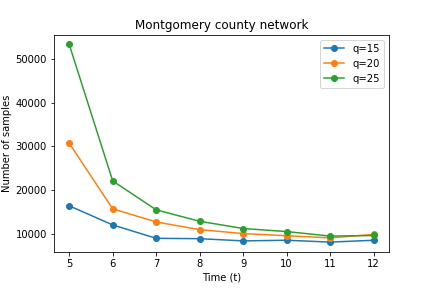
\includegraphics[width=0.3\textwidth]{{figs/montgomery_p0.0435}.png}
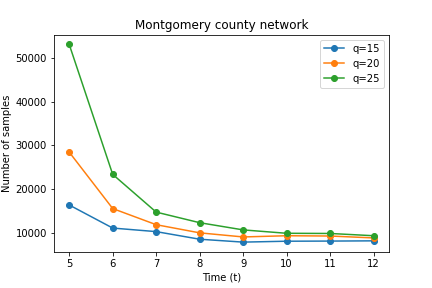
\includegraphics[width=0.3\textwidth]{{figs/montgomery_p0.044}.png}
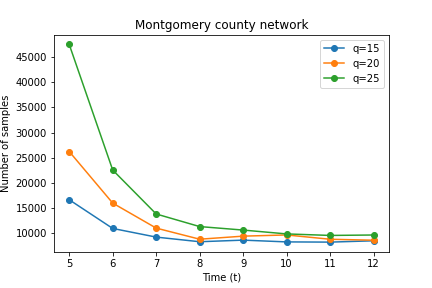
\includegraphics[width=0.3\textwidth]{{figs/montgomery_p0.0445}.png}
\caption{Number of Monte-Carlo samples using the approach of Dagum et al. \cite{dagum:focs95}
on a social contact network for Montgomery county, VA, constructed using the approach of
\cite{eubank:nature04, barrett:wsc09},
for a transmission probability, such that the expected number of infections 
is around 15\% of the total number of nodes with varying
probability values: low (left), medium (middle), and high (right).
}
\label{fig:dagum-mcmc-montgomery}
\end{figure}

\begin{figure}
\centering
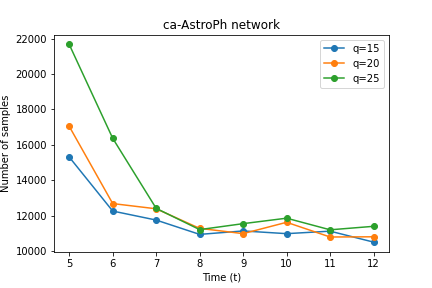
\includegraphics[width=0.3\textwidth]{{figs/ca-AstroPh_p0.0254}.png}
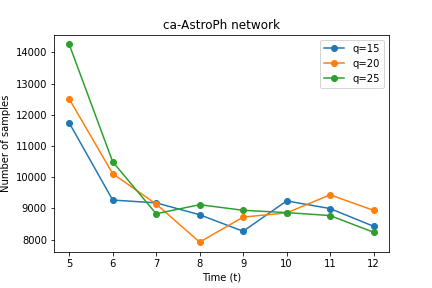
\includegraphics[width=0.3\textwidth]{{figs/ca-AstroPh_p0.03}.png}
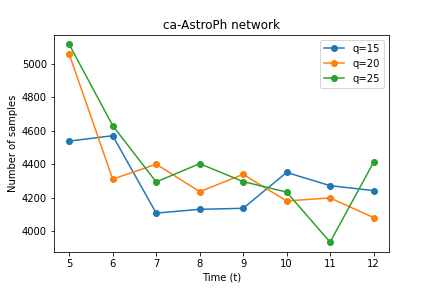
\includegraphics[width=0.3\textwidth]{{figs/ca-AstroPh_p0.06}.png}
\caption{Number of Monte-Carlo samples using the approach of Dagum et al. \cite{dagum:focs95}
for the ca-AstroPh network,
for a transmission probability, such that the expected number of infections 
is around 15\% of the total number of nodes with varying
probability values: low (left), medium (middle), and high (right).
}
\label{fig:dagum-mcmc-ca-astroph}
\end{figure}


\begin{figure}
\centering
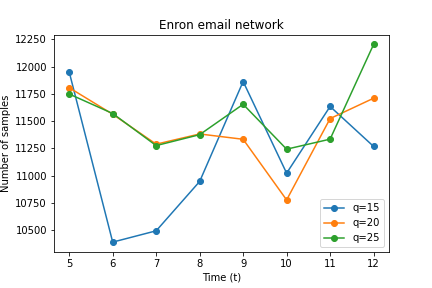
\includegraphics[width=0.3\textwidth]{{figs/email-Enron_p0.0498}.png}
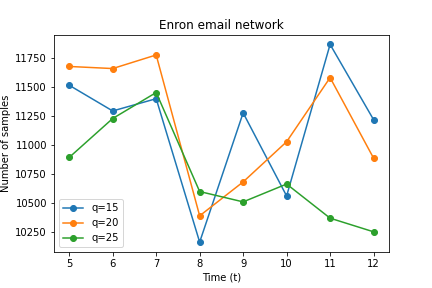
\includegraphics[width=0.3\textwidth]{{figs/email-Enron_p0.0515}.png}
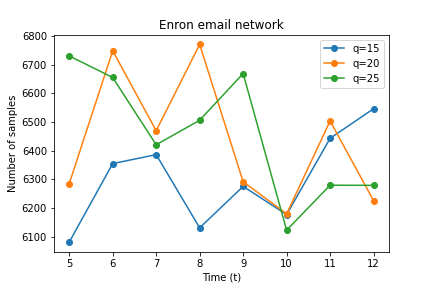
\includegraphics[width=0.3\textwidth]{{figs/email-Enron_p0.098}.png}
\caption{Number of Monte-Carlo samples using the approach of Dagum et al. \cite{dagum:focs95}
for the Enron email network,
for a transmission probability, such that the expected number of infections 
is around 15\% of the total number of nodes with varying
probability values: low (left), medium (middle), and high (right).
}
\label{fig:dagum-mcmc-enron}
\end{figure}


\begin{figure}
\centering
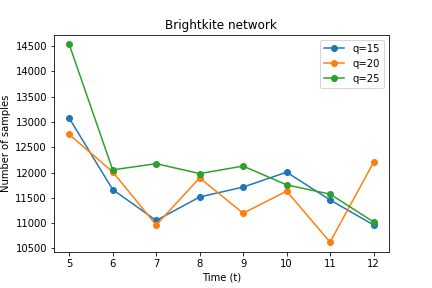
\includegraphics[width=0.3\textwidth]{{figs/loc-brightkite_p0.0693}.png}
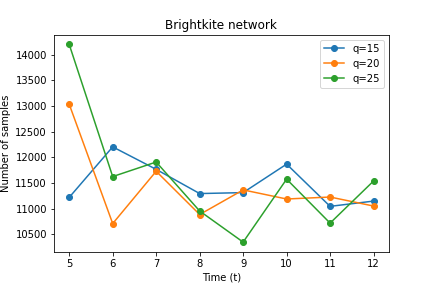
\includegraphics[width=0.3\textwidth]{{figs/loc-brightkite_p0.07045}.png}
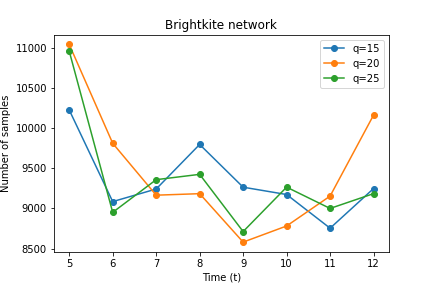
\includegraphics[width=0.3\textwidth]{{figs/loc-brightkite_p0.0852}.png}
\caption{Number of Monte-Carlo samples using the approach of Dagum et al. \cite{dagum:focs95}
for the Brightkite location network,
for a transmission probability, such that the expected number of infections 
is around 15\% of the total number of nodes with varying
probability values: low (left), medium (middle), and high (right).
}
\label{fig:dagum-mcmc-brightkite}
\end{figure}


\begin{figure}
\centering
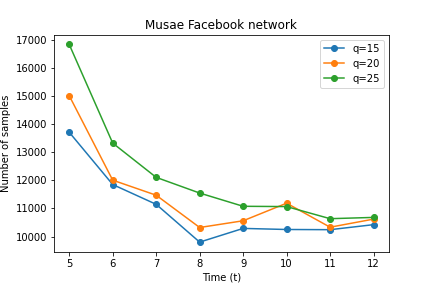
\includegraphics[width=0.3\textwidth]{{figs/musae_facebook_p0.0388}.png}
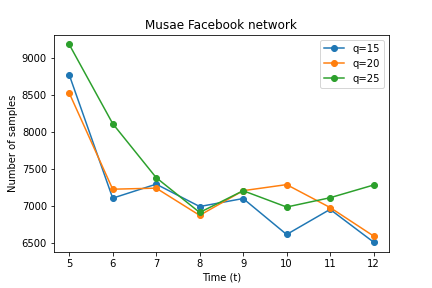
\includegraphics[width=0.3\textwidth]{{figs/musae_facebook_p0.055}.png}
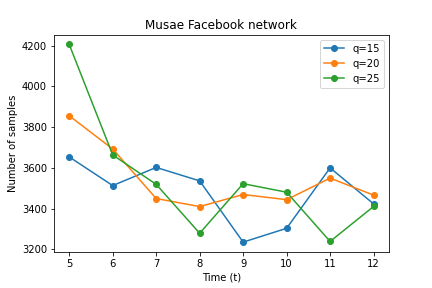
\includegraphics[width=0.3\textwidth]{{figs/musae_facebook_p0.118}.png}
\caption{Number of Monte-Carlo samples using the approach of Dagum et al. \cite{dagum:focs95}
for the Musae Facebook network,
for a transmission probability, such that the expected number of infections 
is around 15\% of the total number of nodes with varying
probability values: low (left), medium (middle), and high (right).
}
\label{fig:dagum-mcmc-facebook}
\end{figure}

